\chapter {Larger Document}

If you are writing a book, it is better to split the book into several parts.

For example:

\begin{verbatim}
  \documentclass{book}
  \usepackage[english]{babel}     
\usepackage[utf8]{inputenc}     % accent symbols
\usepackage[T1]{fontenc}
\usepackage{lmodern}
\usepackage{microtype}
\usepackage{natbib}
\usepackage{tocbibind}          
\usepackage{amsmath}            % math symbols
\usepackage{amsthm}             % math symbols
\usepackage[colorlinks=true,linkcolor=red]{hyperref} % hyper link

% for code
\usepackage{listings}
\usepackage{color,xcolor}
\definecolor{mygreen}{rgb}{0,0.6,0}
\definecolor{mygray}{rgb}{0.9,0.9,0.9}
\definecolor{mymauve}{rgb}{0.58,0,0.82}
\lstset{
backgroundcolor=\color{mygray},
numbers=left,                    
columns=fullflexible,
breaklines=true,      
captionpos=b,         
tabsize=4,            
commentstyle=\color{mygreen}, 
escapeinside={\%*}{*)},       
keywordstyle=\color{blue},    
% stringstyle=\color{mymauve}\monaco,
frame=single,                        
rulesepcolor=\color{red!20!green!20!blue!20},
% identifierstyle=\color{red},
%% language=c++,
basicstyle=\tiny
}

\usepackage{indentfirst}
\setlength{\parindent}{2em}
\usepackage[onehalfspacing]{setspace}
% graph
\usepackage{pdfpages}
\usepackage{graphicx}
% box
\usepackage{booktabs}
\usepackage{tcolorbox}

%% user defined command
\newcommand{\keyword}[1]{\textbf{#1}}
\newcommand{\keywords}[1]{\textbf{#1}}
\newcommand{\lcmd}[1]{\texttt{#1}}
\newcommand{\head}[1]{\textnormal{\textbf{#1}}}
\newcommand{\itwords}[1]{\textit{#1}}

\usepackage{float}
% all symbols
\usepackage{tipa}
\usepackage{tipx}

\usepackage{datetime}
% \usepackage{movie15}


% variable
% TODO
\newcommand{\pdfauthor}{Mike Chyson (Li Mingming)}
\newcommand{\pdftitle}{Principles of Economics}
\newcommand{\pdfsubject}{Principles of Economics}
\newcommand{\pdfkeywords}{Principles of Economics}
\newcommand{\bookname}{Principles of Economics}
\newcommand{\bookoneword}{Citation and interpreation of principles of economics}
\newcommand{\timeandcompany}{Dec, 5, 2020}

\usepackage{bm}
\usepackage{amsfonts}

  \hypersetup{pdfauthor={Li Mingming},
    pdftitle={The Big Book of \LaTeX},
    pdfsubject={Introduction to \LaTeX and how to use it},
    pdfkeywords={latex}}

  \begin{document}

  \frontmatter
  \begin{titlepage}
  \raggedleft
      {\Large 作者\\ 李明明\\[1in] }
  % {\large 关于\\}
  {\Huge\scshape 法语学习\\[.2in]}
  {\large 从零学习法语的笔记整理 \\}
  \vfill
  {\itshape \today{}}
\end{titlepage}


  \chapter*{Dedication}

读《经济学原理》的笔记。

  \tableofcontents
  \listoftables
  \listoffigures
  \mainmatter
  \chapter{Environment}

The operating system is Ubuntu 20.04.1 LTS.

The text editor is Emacs.

The installation of Emacs is as follows:

\lstset{language=sh}
\begin{lstlisting}
  sudo apt install emacs
\end{lstlisting}

The installation of LaTex and some packages is as follows:
\begin{lstlisting}
  sudo apt install texlive-latex-base
  sudo apt install texlive-xetex
  sudo apt install texlive-full
\end{lstlisting}







  \chapter{What is \LaTeX}

\section{What is \LaTeX}
\LaTeX is a document markup language.


\section{\LaTeX's Properties}


\begin{enumerate}
\item \LaTeX is portable in three ways:
  \begin{enumerate}
  \item The source code is open.
  \item The implementation is in plain text.
  \item The output is in multiple format: PDF, DVI, PostScript, HTML.
  \end{enumerate}
\item Protect your work:
  \begin{enumerate}
  \item compatibility (plain text)
  \item no viruses (plain text)
  \end{enumerate}
\end{enumerate}


\section{Reason to Use It}
Becuase \LaTeX is a markup language, you should learn it before you can use it.
So why should you spend so much time to learn it while there is so much document creator like Word, Pages?

There is several reasons that push me to select it:
\begin{description}
  \item[powerful:] \LaTeX provides powerful edit ability. You can almost get whatever you want to show, especially the mathematical equations. Other document editor is less powerful in equations editing.
  \item[easy to alter:] Because \LaTeX seperate the format and the content, it is easy to do format alteration in the full document domain, for example change the style of the capter.
  \item[one for all:] Once you create your own template, it is easy to wreate document with the template applied, saving so much time in format. The disadvantage is that you spend more time in the first time.
\end{description}


  \chapter{\LaTeX Base}
\section{Hello World in \LaTeX}

\lstset{language=TeX}
\begin{lstlisting}
  \documentclass[a4paper,11pt]{article} % specify the document class, different class for different purpose.
  \begin{document}
  \title{Example}
  \author{Mike Chyson}
  \date{Thu Jan  3 16:22:11 CST 2019}
  \maketitle                    % make a title according to the title and author etc.
  \section{What's this?}        
  This is simple document. It contains a title and a section with text.
  \end{document}
\end{lstlisting}

The output is as follows:
%% 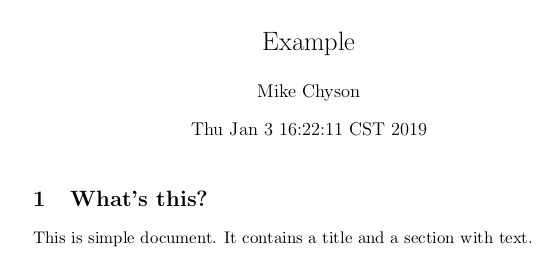
\includepdf[frame=true]{example}
\begin{figure}
  \centering
  \fbox{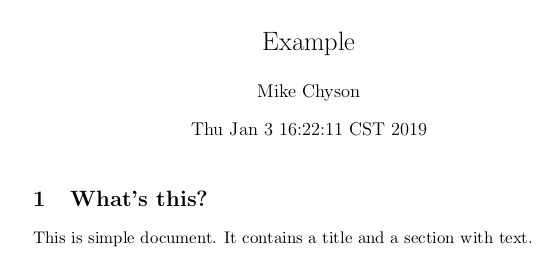
\includegraphics[width=0.8\textwidth]{example.png}}
  \caption{Example}
\end{figure}



Because the seperation of the format and the content, 
you do not specify the font size, font color, font family and so on.
Instead, you tell \LaTeX it is a \lcmd{title}, or \lcmd{author} or \lcmd{date} and so on.
\LaTeX format them for you.
As if there is a logical layer between the appearance and the content.


\section{Document Structure}
A \LaTeX document doesn't stand alone — commonly the document is based on a versatile template.
Such a fundamental template is called a class.
It provides customizable features, usually built for a certain purpose.

This first part of the document is called the preamble of the document. This is where we choose the class, specify properties, and in general, make document-wide definitions.

The first line starts with \verb|\documentclass|.
This word begins with a backslash; such a word is called a \keyword{command}.
We used commands to specify the class and to state document properties: \lcmd{title} , \lcmd{author} , and \lcmd{date}.


\begin{verbatim}
  preamble
  body
\end{verbatim}


\section{\LaTeX Command}
\lstset{language=TeX}
\begin{lstlisting}
  \command
  \command{argument}
  \command[optional argument]{argument}
\end{lstlisting}


\section{Comment}
The percent sing(\%) introduces a \keyword{comment}.




\section{Create Your Own Commands}

\subsection{With No Arguments}
\begin{lstlisting}
  \newcommand{\TUG}{TeX Users Group}
  \TUG
\end{lstlisting}

\subsection{With Arguments}

\begin{lstlisting}
  \newcommand{\keyword}[1]{\textbf{#1}}
  \keyword{declrations}
\end{lstlisting}

\subsection{With Optional Arguments}

\begin{lstlisting}
  \newcommand{\keyword2}[2][\bfseries]{{#1#2}}
  \keyword2[\itshape]{declarations}
\end{lstlisting}


\section{Breaking Lines}
\begin{lstlisting}
  \\                            % end a line
  \newline                      % has the same effect with \\
  \linebreak                    % tells LeTeX to end the line but to keep the full justification
  \\[3mm]                       % insert additional vertical space after the break depending on the value
  \linebreak[4]                 % can be used to influence the line break slightly or strongly:
%% If number is 0, a line break is allowed, 1 means it's desired, 2 and 3 mark more
%% insistent requests, and 4 will force it. The latter is the default behavior if no number
  %% was given.
  \nolinebreak
\end{lstlisting}


\section{Breaking Pages}
\begin{lstlisting}
  \pagebreak
  \newpage
  \nopagebreak
\end{lstlisting}


\section{Get Help}
Three ways to get help about the package:
\begin{itemize}
\item Use the \verb|texdoc| command:
  \begin{lstlisting}
    texdoc <package>
  \end{lstlisting}
\item Use the \verb|kpsewhich| command:
  \begin{lstlisting}
    kpsewhich <package>.sty
  \end{lstlisting}
\item Visit the website: \url{http://ctan.org/pkg}
\end{itemize}

  \chapter{Font}
\section{Shape}
\begin{table}[!h]
  \centering
  \caption{Font Command}
  \begin{tabular}{ccc}
    \toprule[1.5pt]
    \head{Command} & \head{Explaination} & \head{Output} \\
    \midrule
    \verb|\textbf| & bold font & \textbf{Example} \\
    \verb|\textit| & italic & \textit{Example} \\
    \verb|\textsl| & slated & \textsl{Example} \\
    \verb|\textsc| & small caps & \textsc{Example} \\
    \verb|\textup| & & \textup{Example} \\
    \verb|\textmd| & medium & \textmd{Example} \\
    \verb|\textnormal| & & \textnormal{Example} \\
    \bottomrule[1.5pt]
    
  \end{tabular}
  
\end{table}


\begin{table}[!h]
  \centering
  \caption{Font Declaration}
  \begin{tabular}{ccc}
    \toprule[1.5pt]
    \head{Declaration} & \head{Explaination} & \head{Output} \\
    \midrule
    \verb|\itshape| & italic & {\itshape Example} \\
    \verb|\bfseries| & bold font & {\bfseries Example} \\
    \verb|\slshape| & slated & {\slshape Example} \\
    \verb|\scshape| & small caps & {\scshape Example} \\
    \verb|\upshape| & & {\upshape Example} \\
    \verb|\mdseries| & medium & {\mdseries Example} \\
    \verb|\normalfont| & & {\normalfont Example} \\
    \bottomrule[1.5pt]
    
  \end{tabular}
  
\end{table}


\begin{table}[!hbp]
  \centering
  \caption{Font Emphasized}
  \begin{tabular}{ccc}
    \toprule[1.5pt]
    \head{Command} & \head{Explaination} & \head{Output} \\
    \midrule
    \verb|\emph| & emphasized & \emph{Example} \\
    \bottomrule[1.5pt]
  \end{tabular}
\end{table}
\clearpage
\section{Family}
\begin{table}[!hbp]
  \centering
  \caption{Font Family}
  \begin{tabular}{ccc}
    \toprule[1.5pt]
    \head{Command or Declariation} & \head{Explaination} & \head{Output} \\
    \midrule
    \verb|\textsf| & sans-serif & \textsf{Example} \\
    \verb|\texttt| & typewritter & \texttt{Example} \\
    \verb|\textrm| & Roman & \textrm{Example} \\
    \bottomrule[1.5pt]
  \end{tabular}
\end{table}

\clearpage

\section{Size}
\begin{table}[!hbp]
  \centering
  \caption{Font Size}
  \begin{tabular}{cc}
    \toprule[1.5pt]
    \head{Command} & \head{Output} \\
    \midrule
    \verb|\tiny| & \tiny{Example} \\
    \verb|\scriptsize| & \scriptsize{Example} \\
    \verb|\footnotesize| & \footnotesize{Example} \\
    \verb|\small| & \small{Example} \\
    \verb|\normalsize| & \normalsize{Example} \\
    \verb|\large| & \large{Example} \\
    \verb|\Large| & \Large{Example} \\
    \verb|\LARGE| & \LARGE{Example} \\
    \verb|\huge| & \huge{Example} \\
    \verb|\Huge| & \Huge{Example} \\
    \bottomrule[1.5pt]
  \end{tabular}
\end{table}


  

\chapter{Box}

\begin{lstlisting}
  \quad\parbox[b]{1.8cm}{this parbox is aligned at its bottom line}
\end{lstlisting}
\begin{tcolorbox}
\quad\parbox[b]{1.8cm}{this parbox is aligned at its bottom line}  
\end{tcolorbox}


\begin{lstlisting}
  \quad\parbox{1.5cm}{center-aligned parbox}
\end{lstlisting}
\begin{tcolorbox}
\quad\parbox{1.5cm}{center-aligned parbox}  
\end{tcolorbox}


\begin{lstlisting}
  \quad\parbox[t]{2cm}{another parbox aligned at its top line}
\end{lstlisting}
\begin{tcolorbox}
  \quad\parbox[t]{2cm}{another parbox aligned at its top line}
\end{tcolorbox}



\begin{lstlisting}
  \mbox{Hello World}
\end{lstlisting}

\begin{tcolorbox}
  \mbox{Hello World}
\end{tcolorbox}

  \chapter{Justification}
\begin{lstlisting}
\parbox{3cm}{\raggedright hello}    % \raggedright
{\centering hello}            % \centering
\begin{center}                % environment
  hello
\end{center}
\end{lstlisting}



  \chapter{Designing Pages}

\section{Defining the Overall Layout}
\begin{lstlisting}
  \usepackage[a4paper, inner=1.5cm, outer=3cm, top=2cm, bottom=3cm, bindingoffset=1cm, landscape]{geometry}
  %% paper=name
  %% paperwidth=7in
  %% paperheight=10in
  %% papersize={7in,10in}
  %% landscape
  %% portrait
  %% textwidth=140mm
  %% textheight=180mm
  %% lines=25
  %% includedhead % cause the header of the page to be included into the body area
  %% includefoot
  %% left=2cm
  %% right=2cm
  %% bindingoffset % reserves space on the left margin (one-size), respectively the inner margin (two-sided) for the binding

  %% default margin ratio:
  %% top:bottom = 2:3
  %% left:right = 1:1 for one-side documents
  %% inner:outer = 2:3 for two-side documents
\end{lstlisting}

\begin{lstlisting}
  \usepackage[onehalfspacing]{setspace}
  %% singlespacing, onehalfspacing, doublespacing
  %% \begin{spacing}{2.4}
  %% This text is stretched by a factor of 2.4.
  %% \end{spacing}
\end{lstlisting}


\begin{lstlisting}
  \documentclass[a4paper,12pt,twocolumn]{book} % the document class book, suitable for book-like documents
  %% book, report, article, slides, letter
  %% oneside or twoside
  %% openright or openany % only support book and report
  %% titlepage or notitlepage
  %% final or draft: If draft is set, then LaTeX will mark overfull lines with a black box, which is helpful in reviewing and improving the output.
  %% openbib : When this option is set, a bibliography would be formatted in open style instead of compressed style.
  %% fleqn : Causes displayed formulas to be left-aligned.
  %% leqno : For numbered displayed formulas, the number would be put to the left side. The right side is the default.
\end{lstlisting}


\section{Creating a Table of Contents}
\begin{lstlisting}
  \tableofcontents
\end{lstlisting}

\section{Designing Headers and Footers}
\begin{lstlisting}
  \usepackage{fancyhdr}
  \fancyhf{}
  \fancyhead[LE]{\leftmark}
  \fancyhead[RO]{\nouppercase{\rightmark}}
  \fancyfoot[LE,RO]{\thepage}
  \pagestyle{fancy}
\end{lstlisting}

  \chapter{Footnotes}

\begin{lstlisting}
  \footnote{hello world}
  \section[title without footnote]{This is a section\protect\footnote{section footnote}}

  \footnote[number]{text}

  \footnotemark[number] % produces a superscripted number in the text as a
  % footnote mark. If the optional argument wasn't given, it's also stepping and using
  % the internal footnote counter. No footnote will be generated.

  \footnotetext[number]{text} % generates a footnote without putting a
  % footnote mark into the text without stepping the internal footnote counter.

  \footnoterule % used to alter the footnote line

  \renewcommand{\footnoterule}{\noindent\smash{\rule[3pt]{\textwidth}{0.4pt}}}
  % \rule[raising]{width}{height} draws a line, here 0.4 pt thick, and as wide as the text, raised a bit by 3 pt.
  % \smash , let the line pretend to have a height and a depth of zero, so it's occupying no vertical space at all.
\end{lstlisting}

Example:
\begin{lstlisting}
  Hello World\footnote{hello world}
\end{lstlisting}
\begin{tcolorbox}
Hello World\footnote{hello world}.  
\end{tcolorbox}




  \chapter{Lists}
\section{Bulleted Lists}

\begin{lstlisting}
  \begin{itemize}
  \item geometry
  \item amsmath
  \end{itemize}
\end{lstlisting}

\begin{tcolorbox}
  \begin{itemize}
  \item geometry
  \item amsmath
  \end{itemize}
\end{tcolorbox}

\section{Numbered Lists}
\begin{lstlisting}
  \begin{enumerate}
  \item geometry
  \item amsmath
  \end{enumerate}
\end{lstlisting}

\begin{tcolorbox}
  \begin{enumerate}
  \item geometry
  \item amsmath
  \end{enumerate}
\end{tcolorbox}



\section{Definition Lists}
\begin{lstlisting}
  \begin{description}
  \item[paralist] provides compact lists and list versions that
    can be used within paragraphs, helps to customize labels and
    layout
  \item[enumitem] gives control over labels and lengths
    in all kind of lists
  \item[mdwlist] is useful to customize description lists, it
    even allows multi-line labels. It features compact lists and
    the capability to suspend and resume.
  \item[desclist] offers more flexibility in definition list
  \item[multenum] produces vertical enumeration in multiple
    columns
  \end{description}
\end{lstlisting}

\begin{tcolorbox}
  \begin{description}
  \item[paralist] provides compact lists and list versions that
    can be used within paragraphs, helps to customize labels and
    layout
  \item[enumitem] gives control over labels and lengths
    in all kind of lists
  \item[mdwlist] is useful to customize description lists, it
    even allows multi-line labels. It features compact lists and
    the capability to suspend and resume.
  \item[desclist] offers more flexibility in definition list
  \item[multenum] produces vertical enumeration in multiple
    columns
  \end{description}
\end{tcolorbox}

  \chapter{Tables}

\begin{lstlisting}
  \newcommand{\head}[1]{\textnormal{\textbf{#1}}}
  \begin{tabular}{ccc}
    \hline
    \head{Command} & \head{Declaration} & \head{Output} \\
    \hline
    \verb|\textrm| & \verb|\rmfamily| & \rmfamily Example text \\
    \verb|\textsf| & \verb|\sffamily| & \sffamily Example text \\
    \verb|\texttt| & \verb|\ttfamily| & \ttfamily Example text \\
    \hline
  \end{tabular}
\end{lstlisting}

\begin{tcolorbox}
  \begin{tabular}{ccc}
    \hline
    \head{Command} & \head{Declaration} & \head{Output} \\
    \hline
    \verb|\textrm| & \verb|\rmfamily| & \rmfamily Example text \\
    \verb|\textsf| & \verb|\sffamily| & \sffamily Example text \\
    \verb|\texttt| & \verb|\ttfamily| & \ttfamily Example text \\
    \hline
  \end{tabular}
\end{tcolorbox}


\newpage
\begin{lstlisting}

  \usepackage{booktabs} % toprule, midrule, bottomrule

  \begin{tabular}{ccc}
    \toprule[1.5pt] % British typesetters call a line a rule
    \head{Command} & \head{Declaration}& \head{Output}\\
    \midrule %
    \verb|\textrm| & \verb|\rmfamily| & \rmfamily Example text \\
    \verb|\textsf| & \verb|\sffamily| & \sffamily Example text \\
    \verb|\texttt| & \verb|\ttfamily| & \ttfamily Example text \\
    \bottomrule[1.5pt] %
  \end{tabular}

\end{lstlisting}

\begin{tcolorbox}
  
  \begin{tabular}{ccc}
    \toprule[1.5pt] % British typesetters call a line a rule
    \head{Command} & \head{Declaration}& \head{Output}\\
    \midrule %
    \verb|\textrm| & \verb|\rmfamily| & \rmfamily Example text \\
    \verb|\textsf| & \verb|\sffamily| & \sffamily Example text \\
    \verb|\texttt| & \verb|\ttfamily| & \ttfamily Example text \\
    \bottomrule[1.5pt] %
  \end{tabular}

\end{tcolorbox}


\begin{tcolorbox}
  To avoid the table exceed out the page:
\begin{verbatim}
    \resizebox{\textwidth}{!}{
      ...
    }
  
\end{verbatim}


\end{tcolorbox}


To wrap automatically in cell, use the \verb|p{width}| parameter.
For example:
\begin{lstlisting}
  
\begin{table}[htb!]
  \centering
  \begin{tabular}{p{0.3\columnwidth}p{0.3\columnwidth}p{0.3\columnwidth}}
    \toprule{}
    & \head{advantage} & \head{disadvantage} \\
    \midrule
    multiple processes & each process runs independently & communication and data sharing can be inconvenient \\
    multiple threads & can communicate simply by data sharing & more complex than single-threaded program\\
    \bottomrule
  \end{tabular}
  \caption{multiple processes and multiple threads}
\end{table}
\end{lstlisting}


\begin{table}[htb!]
  \centering
  \begin{tabular}{p{0.3\columnwidth}p{0.3\columnwidth}p{0.3\columnwidth}}
    \toprule{}
    & \head{advantage} & \head{disadvantage} \\
    \midrule
    multiple processes & each process runs independently & communication and data sharing can be inconvenient \\
    multiple threads & can communicate simply by data sharing & more complex than single-threaded program\\
    \bottomrule
  \end{tabular}
  \caption{multiple processes and multiple threads}
\end{table}






  \chapter{Figure}

\begin{lstlisting}
  \usepackage{graphicx}
  \begin{figure}
    \centering
    
\includegraphics[width=0.8\textwidth]{zm.jpg}   % include picture
  \end{figure}
\end{lstlisting}


\begin{figure}
  \centering
  
\includegraphics[width=0.8\textwidth]{zm.jpg}   % include picture
\end{figure}





  \chapter{Cross Referencing}
\begin{lstlisting}
  \label % mark the label
  \ref % refer after marking
  \pageref
  % notice, typeset twice to produce the corrent reference

  % If the \label command appeared in ordinary text, then the current sectional unit,
  % like the chapter or the section, would be assigned.
  % If the \label would be placed within a numbered environment, that environment
  % would be assigned to the key.

  \newcommand{\fullref}[1]{\ref{#1} on page~\pageref{#1}}
\end{lstlisting}

For example:

\begin{lstlisting}
  Hello World\label{hello-label}

  Refer to \ref{hello-label}
\end{lstlisting}

\begin{tcolorbox}
Hello World\label{hello-label}

Refer to \ref{hello-label}
\end{tcolorbox}


  \chapter{Content}

\begin{table}[!ht]
  \caption{Content}
  \centering
  \begin{tabular}{cc}
    \toprule[1.5pt]
    \head{Command} & \head{Level} \\
    \midrule
    \verb|\part| & -1 (book and report class) \\
    \verb|\chapter| & 0 (not available in article) \\
    \verb|\section| & 1 \\
    \verb|\subsection| & 2 \\
    \verb|\subsubsection| & 3 \\
    \verb|\paragraph| & 4 \\
    \verb|\subparagraph| & 5 \\
    \bottomrule[1.5pt]
  \end{tabular}
\end{table}



  \chapter{Math}

\section{Basic Formula}

\begin{lstlisting}
  \section*{Quadratic equations}
  \begin{equation}
    \label{quad}
    ax^2 + bx + c = 0,
  \end{equation}
  where \( a, b\) and \( c \) are constants and \( a \neq 0 \),
  has two solutions for the variable \( x \):
  \begin{equation}
    \label{root}
    x_{1,2} = \frac{-b \pm \sqrt{b^2 -4ac}}{2a}.
  \end{equation}
  If the \emph{discriminant} \( \Detla \) with
  \[ \Delta = b^2 - 4ac \]
  is zero, then the equation (\ref{quad}) has a double solution:
  (\ref{root}) becomes
  \[ x = - \frac{b}{2a}. \]
\end{lstlisting}

% \begin{tcolorbox}
%   \section*{Quadratic equations}
%   \begin{equation}
%     \label{quad}
%     ax^2 + bx + c = 0,
%   \end{equation}
%   where \( a, b\) and \( c \) are constants and \( a \neq 0 \),
%   has two solutions for the variable \( x \):
%   \begin{equation}
%     \label{root}
%     x_{1,2} = \frac{-b \pm \sqrt{b^2 -4ac}}{2a}.
%   \end{equation}
%   If the \emph{discriminant} \( \Detla \) with
%   \[ \Delta = b^2 - 4ac \]
%   is zero, then the equation (\ref{quad}) has a double solution:
%   (\ref{root}) becomes
%   \[ x = - \frac{b}{2a}. \]

% \end{tcolorbox}


\section{Expressions within Text}
LaTeX provides the math environment in-text formulas:

\begin{lstlisting}
  \begin{math}
    expression
  \end{math}
\end{lstlisting}

LaTeX offers an alias that's doing the same:

\begin{lstlisting}
  \( expression \)
\end{lstlisting}

A third way is by using a shortcut, coming from TeX:

\begin{lstlisting}
  $expression$
\end{lstlisting}

For example:
\begin{tcolorbox}
  \begin{lstlisting}
    This is an equation: $x^2 + x = 10$
  \end{lstlisting}
  This is an equation: $x^2 + x = 10$
\end{tcolorbox}

\section{Displaying Formula}

\begin{lstlisting}
  \begin{displaymath}
    expression                  % displayed formula, centered
  \end{displaymath}
\end{lstlisting}


There are shortcuts:
\begin{lstlisting}
  \[
    expression
  \]
\end{lstlisting}

\begin{lstlisting}
  $$
  expression
  $$
\end{lstlisting}



For example:
\begin{tcolorbox}
  \begin{lstlisting}
    \begin{displaymath}
      x^2 + x = 10
    \end{displaymath}
  \end{lstlisting}
  \begin{displaymath}
    x^2 + x = 10
  \end{displaymath}

\end{tcolorbox}


\section{Numbering Equations}
\begin{tcolorbox}
  \begin{lstlisting}
    \begin{equation}
      \label{newton}
      F = ma^2
    \end{equation}
    Newton's law: \eqref{newton}.
  \end{lstlisting}
  \begin{equation}
    \label{newton}
    F = ma^2
  \end{equation}
  Newton's law: \eqref{newton}.

\end{tcolorbox}



  \chapter {Larger Document}

If you are writing a book, it is better to split the book into several parts.

For example:

\begin{verbatim}
  \documentclass{book}
  \usepackage[english]{babel}     
\usepackage[utf8]{inputenc}     % accent symbols
\usepackage[T1]{fontenc}
\usepackage{lmodern}
\usepackage{microtype}
\usepackage{natbib}
\usepackage{tocbibind}          
\usepackage{amsmath}            % math symbols
\usepackage{amsthm}             % math symbols
\usepackage[colorlinks=true,linkcolor=red]{hyperref} % hyper link

% for code
\usepackage{listings}
\usepackage{color,xcolor}
\definecolor{mygreen}{rgb}{0,0.6,0}
\definecolor{mygray}{rgb}{0.9,0.9,0.9}
\definecolor{mymauve}{rgb}{0.58,0,0.82}
\lstset{
backgroundcolor=\color{mygray},
numbers=left,                    
columns=fullflexible,
breaklines=true,      
captionpos=b,         
tabsize=4,            
commentstyle=\color{mygreen}, 
escapeinside={\%*}{*)},       
keywordstyle=\color{blue},    
% stringstyle=\color{mymauve}\monaco,
frame=single,                        
rulesepcolor=\color{red!20!green!20!blue!20},
% identifierstyle=\color{red},
%% language=c++,
basicstyle=\tiny
}

\usepackage{indentfirst}
\setlength{\parindent}{2em}
\usepackage[onehalfspacing]{setspace}
% graph
\usepackage{pdfpages}
\usepackage{graphicx}
% box
\usepackage{booktabs}
\usepackage{tcolorbox}

%% user defined command
\newcommand{\keyword}[1]{\textbf{#1}}
\newcommand{\keywords}[1]{\textbf{#1}}
\newcommand{\lcmd}[1]{\texttt{#1}}
\newcommand{\head}[1]{\textnormal{\textbf{#1}}}
\newcommand{\itwords}[1]{\textit{#1}}

\usepackage{float}
% all symbols
\usepackage{tipa}
\usepackage{tipx}

\usepackage{datetime}
% \usepackage{movie15}


% variable
% TODO
\newcommand{\pdfauthor}{Mike Chyson (Li Mingming)}
\newcommand{\pdftitle}{Principles of Economics}
\newcommand{\pdfsubject}{Principles of Economics}
\newcommand{\pdfkeywords}{Principles of Economics}
\newcommand{\bookname}{Principles of Economics}
\newcommand{\bookoneword}{Citation and interpreation of principles of economics}
\newcommand{\timeandcompany}{Dec, 5, 2020}

\usepackage{bm}
\usepackage{amsfonts}

  \hypersetup{pdfauthor={Li Mingming},
    pdftitle={The Big Book of \LaTeX},
    pdfsubject={Introduction to \LaTeX and how to use it},
    pdfkeywords={latex}}

  \begin{document}

  \frontmatter
  \begin{titlepage}
  \raggedleft
      {\Large 作者\\ 李明明\\[1in] }
  % {\large 关于\\}
  {\Huge\scshape 法语学习\\[.2in]}
  {\large 从零学习法语的笔记整理 \\}
  \vfill
  {\itshape \today{}}
\end{titlepage}


  \chapter*{Dedication}

读《经济学原理》的笔记。

  \tableofcontents
  \listoftables
  \listoffigures
  \mainmatter
  \chapter{Environment}

The operating system is Ubuntu 20.04.1 LTS.

The text editor is Emacs.

The installation of Emacs is as follows:

\lstset{language=sh}
\begin{lstlisting}
  sudo apt install emacs
\end{lstlisting}

The installation of LaTex and some packages is as follows:
\begin{lstlisting}
  sudo apt install texlive-latex-base
  sudo apt install texlive-xetex
  sudo apt install texlive-full
\end{lstlisting}







  \chapter{What is \LaTeX}

\section{What is \LaTeX}
\LaTeX is a document markup language.


\section{\LaTeX's Properties}


\begin{enumerate}
\item \LaTeX is portable in three ways:
  \begin{enumerate}
  \item The source code is open.
  \item The implementation is in plain text.
  \item The output is in multiple format: PDF, DVI, PostScript, HTML.
  \end{enumerate}
\item Protect your work:
  \begin{enumerate}
  \item compatibility (plain text)
  \item no viruses (plain text)
  \end{enumerate}
\end{enumerate}


\section{Reason to Use It}
Becuase \LaTeX is a markup language, you should learn it before you can use it.
So why should you spend so much time to learn it while there is so much document creator like Word, Pages?

There is several reasons that push me to select it:
\begin{description}
  \item[powerful:] \LaTeX provides powerful edit ability. You can almost get whatever you want to show, especially the mathematical equations. Other document editor is less powerful in equations editing.
  \item[easy to alter:] Because \LaTeX seperate the format and the content, it is easy to do format alteration in the full document domain, for example change the style of the capter.
  \item[one for all:] Once you create your own template, it is easy to wreate document with the template applied, saving so much time in format. The disadvantage is that you spend more time in the first time.
\end{description}


  \chapter{\LaTeX Base}
\section{Hello World in \LaTeX}

\lstset{language=TeX}
\begin{lstlisting}
  \documentclass[a4paper,11pt]{article} % specify the document class, different class for different purpose.
  \begin{document}
  \title{Example}
  \author{Mike Chyson}
  \date{Thu Jan  3 16:22:11 CST 2019}
  \maketitle                    % make a title according to the title and author etc.
  \section{What's this?}        
  This is simple document. It contains a title and a section with text.
  \end{document}
\end{lstlisting}

The output is as follows:
%% 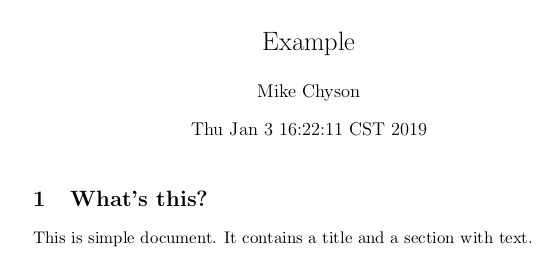
\includepdf[frame=true]{example}
\begin{figure}
  \centering
  \fbox{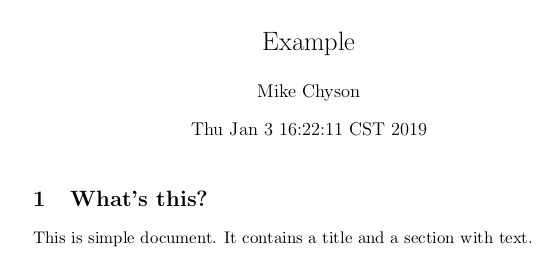
\includegraphics[width=0.8\textwidth]{example.png}}
  \caption{Example}
\end{figure}



Because the seperation of the format and the content, 
you do not specify the font size, font color, font family and so on.
Instead, you tell \LaTeX it is a \lcmd{title}, or \lcmd{author} or \lcmd{date} and so on.
\LaTeX format them for you.
As if there is a logical layer between the appearance and the content.


\section{Document Structure}
A \LaTeX document doesn't stand alone — commonly the document is based on a versatile template.
Such a fundamental template is called a class.
It provides customizable features, usually built for a certain purpose.

This first part of the document is called the preamble of the document. This is where we choose the class, specify properties, and in general, make document-wide definitions.

The first line starts with \verb|\documentclass|.
This word begins with a backslash; such a word is called a \keyword{command}.
We used commands to specify the class and to state document properties: \lcmd{title} , \lcmd{author} , and \lcmd{date}.


\begin{verbatim}
  preamble
  body
\end{verbatim}


\section{\LaTeX Command}
\lstset{language=TeX}
\begin{lstlisting}
  \command
  \command{argument}
  \command[optional argument]{argument}
\end{lstlisting}


\section{Comment}
The percent sing(\%) introduces a \keyword{comment}.




\section{Create Your Own Commands}

\subsection{With No Arguments}
\begin{lstlisting}
  \newcommand{\TUG}{TeX Users Group}
  \TUG
\end{lstlisting}

\subsection{With Arguments}

\begin{lstlisting}
  \newcommand{\keyword}[1]{\textbf{#1}}
  \keyword{declrations}
\end{lstlisting}

\subsection{With Optional Arguments}

\begin{lstlisting}
  \newcommand{\keyword2}[2][\bfseries]{{#1#2}}
  \keyword2[\itshape]{declarations}
\end{lstlisting}


\section{Breaking Lines}
\begin{lstlisting}
  \\                            % end a line
  \newline                      % has the same effect with \\
  \linebreak                    % tells LeTeX to end the line but to keep the full justification
  \\[3mm]                       % insert additional vertical space after the break depending on the value
  \linebreak[4]                 % can be used to influence the line break slightly or strongly:
%% If number is 0, a line break is allowed, 1 means it's desired, 2 and 3 mark more
%% insistent requests, and 4 will force it. The latter is the default behavior if no number
  %% was given.
  \nolinebreak
\end{lstlisting}


\section{Breaking Pages}
\begin{lstlisting}
  \pagebreak
  \newpage
  \nopagebreak
\end{lstlisting}


\section{Get Help}
Three ways to get help about the package:
\begin{itemize}
\item Use the \verb|texdoc| command:
  \begin{lstlisting}
    texdoc <package>
  \end{lstlisting}
\item Use the \verb|kpsewhich| command:
  \begin{lstlisting}
    kpsewhich <package>.sty
  \end{lstlisting}
\item Visit the website: \url{http://ctan.org/pkg}
\end{itemize}

  \chapter{Font}
\section{Shape}
\begin{table}[!h]
  \centering
  \caption{Font Command}
  \begin{tabular}{ccc}
    \toprule[1.5pt]
    \head{Command} & \head{Explaination} & \head{Output} \\
    \midrule
    \verb|\textbf| & bold font & \textbf{Example} \\
    \verb|\textit| & italic & \textit{Example} \\
    \verb|\textsl| & slated & \textsl{Example} \\
    \verb|\textsc| & small caps & \textsc{Example} \\
    \verb|\textup| & & \textup{Example} \\
    \verb|\textmd| & medium & \textmd{Example} \\
    \verb|\textnormal| & & \textnormal{Example} \\
    \bottomrule[1.5pt]
    
  \end{tabular}
  
\end{table}


\begin{table}[!h]
  \centering
  \caption{Font Declaration}
  \begin{tabular}{ccc}
    \toprule[1.5pt]
    \head{Declaration} & \head{Explaination} & \head{Output} \\
    \midrule
    \verb|\itshape| & italic & {\itshape Example} \\
    \verb|\bfseries| & bold font & {\bfseries Example} \\
    \verb|\slshape| & slated & {\slshape Example} \\
    \verb|\scshape| & small caps & {\scshape Example} \\
    \verb|\upshape| & & {\upshape Example} \\
    \verb|\mdseries| & medium & {\mdseries Example} \\
    \verb|\normalfont| & & {\normalfont Example} \\
    \bottomrule[1.5pt]
    
  \end{tabular}
  
\end{table}


\begin{table}[!hbp]
  \centering
  \caption{Font Emphasized}
  \begin{tabular}{ccc}
    \toprule[1.5pt]
    \head{Command} & \head{Explaination} & \head{Output} \\
    \midrule
    \verb|\emph| & emphasized & \emph{Example} \\
    \bottomrule[1.5pt]
  \end{tabular}
\end{table}
\clearpage
\section{Family}
\begin{table}[!hbp]
  \centering
  \caption{Font Family}
  \begin{tabular}{ccc}
    \toprule[1.5pt]
    \head{Command or Declariation} & \head{Explaination} & \head{Output} \\
    \midrule
    \verb|\textsf| & sans-serif & \textsf{Example} \\
    \verb|\texttt| & typewritter & \texttt{Example} \\
    \verb|\textrm| & Roman & \textrm{Example} \\
    \bottomrule[1.5pt]
  \end{tabular}
\end{table}

\clearpage

\section{Size}
\begin{table}[!hbp]
  \centering
  \caption{Font Size}
  \begin{tabular}{cc}
    \toprule[1.5pt]
    \head{Command} & \head{Output} \\
    \midrule
    \verb|\tiny| & \tiny{Example} \\
    \verb|\scriptsize| & \scriptsize{Example} \\
    \verb|\footnotesize| & \footnotesize{Example} \\
    \verb|\small| & \small{Example} \\
    \verb|\normalsize| & \normalsize{Example} \\
    \verb|\large| & \large{Example} \\
    \verb|\Large| & \Large{Example} \\
    \verb|\LARGE| & \LARGE{Example} \\
    \verb|\huge| & \huge{Example} \\
    \verb|\Huge| & \Huge{Example} \\
    \bottomrule[1.5pt]
  \end{tabular}
\end{table}


  

\chapter{Box}

\begin{lstlisting}
  \quad\parbox[b]{1.8cm}{this parbox is aligned at its bottom line}
\end{lstlisting}
\begin{tcolorbox}
\quad\parbox[b]{1.8cm}{this parbox is aligned at its bottom line}  
\end{tcolorbox}


\begin{lstlisting}
  \quad\parbox{1.5cm}{center-aligned parbox}
\end{lstlisting}
\begin{tcolorbox}
\quad\parbox{1.5cm}{center-aligned parbox}  
\end{tcolorbox}


\begin{lstlisting}
  \quad\parbox[t]{2cm}{another parbox aligned at its top line}
\end{lstlisting}
\begin{tcolorbox}
  \quad\parbox[t]{2cm}{another parbox aligned at its top line}
\end{tcolorbox}



\begin{lstlisting}
  \mbox{Hello World}
\end{lstlisting}

\begin{tcolorbox}
  \mbox{Hello World}
\end{tcolorbox}

  \chapter{Justification}
\begin{lstlisting}
\parbox{3cm}{\raggedright hello}    % \raggedright
{\centering hello}            % \centering
\begin{center}                % environment
  hello
\end{center}
\end{lstlisting}



  \chapter{Designing Pages}

\section{Defining the Overall Layout}
\begin{lstlisting}
  \usepackage[a4paper, inner=1.5cm, outer=3cm, top=2cm, bottom=3cm, bindingoffset=1cm, landscape]{geometry}
  %% paper=name
  %% paperwidth=7in
  %% paperheight=10in
  %% papersize={7in,10in}
  %% landscape
  %% portrait
  %% textwidth=140mm
  %% textheight=180mm
  %% lines=25
  %% includedhead % cause the header of the page to be included into the body area
  %% includefoot
  %% left=2cm
  %% right=2cm
  %% bindingoffset % reserves space on the left margin (one-size), respectively the inner margin (two-sided) for the binding

  %% default margin ratio:
  %% top:bottom = 2:3
  %% left:right = 1:1 for one-side documents
  %% inner:outer = 2:3 for two-side documents
\end{lstlisting}

\begin{lstlisting}
  \usepackage[onehalfspacing]{setspace}
  %% singlespacing, onehalfspacing, doublespacing
  %% \begin{spacing}{2.4}
  %% This text is stretched by a factor of 2.4.
  %% \end{spacing}
\end{lstlisting}


\begin{lstlisting}
  \documentclass[a4paper,12pt,twocolumn]{book} % the document class book, suitable for book-like documents
  %% book, report, article, slides, letter
  %% oneside or twoside
  %% openright or openany % only support book and report
  %% titlepage or notitlepage
  %% final or draft: If draft is set, then LaTeX will mark overfull lines with a black box, which is helpful in reviewing and improving the output.
  %% openbib : When this option is set, a bibliography would be formatted in open style instead of compressed style.
  %% fleqn : Causes displayed formulas to be left-aligned.
  %% leqno : For numbered displayed formulas, the number would be put to the left side. The right side is the default.
\end{lstlisting}


\section{Creating a Table of Contents}
\begin{lstlisting}
  \tableofcontents
\end{lstlisting}

\section{Designing Headers and Footers}
\begin{lstlisting}
  \usepackage{fancyhdr}
  \fancyhf{}
  \fancyhead[LE]{\leftmark}
  \fancyhead[RO]{\nouppercase{\rightmark}}
  \fancyfoot[LE,RO]{\thepage}
  \pagestyle{fancy}
\end{lstlisting}

  \chapter{Footnotes}

\begin{lstlisting}
  \footnote{hello world}
  \section[title without footnote]{This is a section\protect\footnote{section footnote}}

  \footnote[number]{text}

  \footnotemark[number] % produces a superscripted number in the text as a
  % footnote mark. If the optional argument wasn't given, it's also stepping and using
  % the internal footnote counter. No footnote will be generated.

  \footnotetext[number]{text} % generates a footnote without putting a
  % footnote mark into the text without stepping the internal footnote counter.

  \footnoterule % used to alter the footnote line

  \renewcommand{\footnoterule}{\noindent\smash{\rule[3pt]{\textwidth}{0.4pt}}}
  % \rule[raising]{width}{height} draws a line, here 0.4 pt thick, and as wide as the text, raised a bit by 3 pt.
  % \smash , let the line pretend to have a height and a depth of zero, so it's occupying no vertical space at all.
\end{lstlisting}

Example:
\begin{lstlisting}
  Hello World\footnote{hello world}
\end{lstlisting}
\begin{tcolorbox}
Hello World\footnote{hello world}.  
\end{tcolorbox}




  \chapter{Lists}
\section{Bulleted Lists}

\begin{lstlisting}
  \begin{itemize}
  \item geometry
  \item amsmath
  \end{itemize}
\end{lstlisting}

\begin{tcolorbox}
  \begin{itemize}
  \item geometry
  \item amsmath
  \end{itemize}
\end{tcolorbox}

\section{Numbered Lists}
\begin{lstlisting}
  \begin{enumerate}
  \item geometry
  \item amsmath
  \end{enumerate}
\end{lstlisting}

\begin{tcolorbox}
  \begin{enumerate}
  \item geometry
  \item amsmath
  \end{enumerate}
\end{tcolorbox}



\section{Definition Lists}
\begin{lstlisting}
  \begin{description}
  \item[paralist] provides compact lists and list versions that
    can be used within paragraphs, helps to customize labels and
    layout
  \item[enumitem] gives control over labels and lengths
    in all kind of lists
  \item[mdwlist] is useful to customize description lists, it
    even allows multi-line labels. It features compact lists and
    the capability to suspend and resume.
  \item[desclist] offers more flexibility in definition list
  \item[multenum] produces vertical enumeration in multiple
    columns
  \end{description}
\end{lstlisting}

\begin{tcolorbox}
  \begin{description}
  \item[paralist] provides compact lists and list versions that
    can be used within paragraphs, helps to customize labels and
    layout
  \item[enumitem] gives control over labels and lengths
    in all kind of lists
  \item[mdwlist] is useful to customize description lists, it
    even allows multi-line labels. It features compact lists and
    the capability to suspend and resume.
  \item[desclist] offers more flexibility in definition list
  \item[multenum] produces vertical enumeration in multiple
    columns
  \end{description}
\end{tcolorbox}

  \chapter{Tables}

\begin{lstlisting}
  \newcommand{\head}[1]{\textnormal{\textbf{#1}}}
  \begin{tabular}{ccc}
    \hline
    \head{Command} & \head{Declaration} & \head{Output} \\
    \hline
    \verb|\textrm| & \verb|\rmfamily| & \rmfamily Example text \\
    \verb|\textsf| & \verb|\sffamily| & \sffamily Example text \\
    \verb|\texttt| & \verb|\ttfamily| & \ttfamily Example text \\
    \hline
  \end{tabular}
\end{lstlisting}

\begin{tcolorbox}
  \begin{tabular}{ccc}
    \hline
    \head{Command} & \head{Declaration} & \head{Output} \\
    \hline
    \verb|\textrm| & \verb|\rmfamily| & \rmfamily Example text \\
    \verb|\textsf| & \verb|\sffamily| & \sffamily Example text \\
    \verb|\texttt| & \verb|\ttfamily| & \ttfamily Example text \\
    \hline
  \end{tabular}
\end{tcolorbox}


\newpage
\begin{lstlisting}

  \usepackage{booktabs} % toprule, midrule, bottomrule

  \begin{tabular}{ccc}
    \toprule[1.5pt] % British typesetters call a line a rule
    \head{Command} & \head{Declaration}& \head{Output}\\
    \midrule %
    \verb|\textrm| & \verb|\rmfamily| & \rmfamily Example text \\
    \verb|\textsf| & \verb|\sffamily| & \sffamily Example text \\
    \verb|\texttt| & \verb|\ttfamily| & \ttfamily Example text \\
    \bottomrule[1.5pt] %
  \end{tabular}

\end{lstlisting}

\begin{tcolorbox}
  
  \begin{tabular}{ccc}
    \toprule[1.5pt] % British typesetters call a line a rule
    \head{Command} & \head{Declaration}& \head{Output}\\
    \midrule %
    \verb|\textrm| & \verb|\rmfamily| & \rmfamily Example text \\
    \verb|\textsf| & \verb|\sffamily| & \sffamily Example text \\
    \verb|\texttt| & \verb|\ttfamily| & \ttfamily Example text \\
    \bottomrule[1.5pt] %
  \end{tabular}

\end{tcolorbox}


\begin{tcolorbox}
  To avoid the table exceed out the page:
\begin{verbatim}
    \resizebox{\textwidth}{!}{
      ...
    }
  
\end{verbatim}


\end{tcolorbox}


To wrap automatically in cell, use the \verb|p{width}| parameter.
For example:
\begin{lstlisting}
  
\begin{table}[htb!]
  \centering
  \begin{tabular}{p{0.3\columnwidth}p{0.3\columnwidth}p{0.3\columnwidth}}
    \toprule{}
    & \head{advantage} & \head{disadvantage} \\
    \midrule
    multiple processes & each process runs independently & communication and data sharing can be inconvenient \\
    multiple threads & can communicate simply by data sharing & more complex than single-threaded program\\
    \bottomrule
  \end{tabular}
  \caption{multiple processes and multiple threads}
\end{table}
\end{lstlisting}


\begin{table}[htb!]
  \centering
  \begin{tabular}{p{0.3\columnwidth}p{0.3\columnwidth}p{0.3\columnwidth}}
    \toprule{}
    & \head{advantage} & \head{disadvantage} \\
    \midrule
    multiple processes & each process runs independently & communication and data sharing can be inconvenient \\
    multiple threads & can communicate simply by data sharing & more complex than single-threaded program\\
    \bottomrule
  \end{tabular}
  \caption{multiple processes and multiple threads}
\end{table}






  \chapter{Figure}

\begin{lstlisting}
  \usepackage{graphicx}
  \begin{figure}
    \centering
    
\includegraphics[width=0.8\textwidth]{zm.jpg}   % include picture
  \end{figure}
\end{lstlisting}


\begin{figure}
  \centering
  
\includegraphics[width=0.8\textwidth]{zm.jpg}   % include picture
\end{figure}





  \chapter{Cross Referencing}
\begin{lstlisting}
  \label % mark the label
  \ref % refer after marking
  \pageref
  % notice, typeset twice to produce the corrent reference

  % If the \label command appeared in ordinary text, then the current sectional unit,
  % like the chapter or the section, would be assigned.
  % If the \label would be placed within a numbered environment, that environment
  % would be assigned to the key.

  \newcommand{\fullref}[1]{\ref{#1} on page~\pageref{#1}}
\end{lstlisting}

For example:

\begin{lstlisting}
  Hello World\label{hello-label}

  Refer to \ref{hello-label}
\end{lstlisting}

\begin{tcolorbox}
Hello World\label{hello-label}

Refer to \ref{hello-label}
\end{tcolorbox}


  \chapter{Content}

\begin{table}[!ht]
  \caption{Content}
  \centering
  \begin{tabular}{cc}
    \toprule[1.5pt]
    \head{Command} & \head{Level} \\
    \midrule
    \verb|\part| & -1 (book and report class) \\
    \verb|\chapter| & 0 (not available in article) \\
    \verb|\section| & 1 \\
    \verb|\subsection| & 2 \\
    \verb|\subsubsection| & 3 \\
    \verb|\paragraph| & 4 \\
    \verb|\subparagraph| & 5 \\
    \bottomrule[1.5pt]
  \end{tabular}
\end{table}



  \chapter{Math}

\section{Basic Formula}

\begin{lstlisting}
  \section*{Quadratic equations}
  \begin{equation}
    \label{quad}
    ax^2 + bx + c = 0,
  \end{equation}
  where \( a, b\) and \( c \) are constants and \( a \neq 0 \),
  has two solutions for the variable \( x \):
  \begin{equation}
    \label{root}
    x_{1,2} = \frac{-b \pm \sqrt{b^2 -4ac}}{2a}.
  \end{equation}
  If the \emph{discriminant} \( \Detla \) with
  \[ \Delta = b^2 - 4ac \]
  is zero, then the equation (\ref{quad}) has a double solution:
  (\ref{root}) becomes
  \[ x = - \frac{b}{2a}. \]
\end{lstlisting}

% \begin{tcolorbox}
%   \section*{Quadratic equations}
%   \begin{equation}
%     \label{quad}
%     ax^2 + bx + c = 0,
%   \end{equation}
%   where \( a, b\) and \( c \) are constants and \( a \neq 0 \),
%   has two solutions for the variable \( x \):
%   \begin{equation}
%     \label{root}
%     x_{1,2} = \frac{-b \pm \sqrt{b^2 -4ac}}{2a}.
%   \end{equation}
%   If the \emph{discriminant} \( \Detla \) with
%   \[ \Delta = b^2 - 4ac \]
%   is zero, then the equation (\ref{quad}) has a double solution:
%   (\ref{root}) becomes
%   \[ x = - \frac{b}{2a}. \]

% \end{tcolorbox}


\section{Expressions within Text}
LaTeX provides the math environment in-text formulas:

\begin{lstlisting}
  \begin{math}
    expression
  \end{math}
\end{lstlisting}

LaTeX offers an alias that's doing the same:

\begin{lstlisting}
  \( expression \)
\end{lstlisting}

A third way is by using a shortcut, coming from TeX:

\begin{lstlisting}
  $expression$
\end{lstlisting}

For example:
\begin{tcolorbox}
  \begin{lstlisting}
    This is an equation: $x^2 + x = 10$
  \end{lstlisting}
  This is an equation: $x^2 + x = 10$
\end{tcolorbox}

\section{Displaying Formula}

\begin{lstlisting}
  \begin{displaymath}
    expression                  % displayed formula, centered
  \end{displaymath}
\end{lstlisting}


There are shortcuts:
\begin{lstlisting}
  \[
    expression
  \]
\end{lstlisting}

\begin{lstlisting}
  $$
  expression
  $$
\end{lstlisting}



For example:
\begin{tcolorbox}
  \begin{lstlisting}
    \begin{displaymath}
      x^2 + x = 10
    \end{displaymath}
  \end{lstlisting}
  \begin{displaymath}
    x^2 + x = 10
  \end{displaymath}

\end{tcolorbox}


\section{Numbering Equations}
\begin{tcolorbox}
  \begin{lstlisting}
    \begin{equation}
      \label{newton}
      F = ma^2
    \end{equation}
    Newton's law: \eqref{newton}.
  \end{lstlisting}
  \begin{equation}
    \label{newton}
    F = ma^2
  \end{equation}
  Newton's law: \eqref{newton}.

\end{tcolorbox}



  \chapter {Larger Document}

If you are writing a book, it is better to split the book into several parts.

For example:

\begin{verbatim}
  \documentclass{book}
  \usepackage[english]{babel}     
\usepackage[utf8]{inputenc}     % accent symbols
\usepackage[T1]{fontenc}
\usepackage{lmodern}
\usepackage{microtype}
\usepackage{natbib}
\usepackage{tocbibind}          
\usepackage{amsmath}            % math symbols
\usepackage{amsthm}             % math symbols
\usepackage[colorlinks=true,linkcolor=red]{hyperref} % hyper link

% for code
\usepackage{listings}
\usepackage{color,xcolor}
\definecolor{mygreen}{rgb}{0,0.6,0}
\definecolor{mygray}{rgb}{0.9,0.9,0.9}
\definecolor{mymauve}{rgb}{0.58,0,0.82}
\lstset{
backgroundcolor=\color{mygray},
numbers=left,                    
columns=fullflexible,
breaklines=true,      
captionpos=b,         
tabsize=4,            
commentstyle=\color{mygreen}, 
escapeinside={\%*}{*)},       
keywordstyle=\color{blue},    
% stringstyle=\color{mymauve}\monaco,
frame=single,                        
rulesepcolor=\color{red!20!green!20!blue!20},
% identifierstyle=\color{red},
%% language=c++,
basicstyle=\tiny
}

\usepackage{indentfirst}
\setlength{\parindent}{2em}
\usepackage[onehalfspacing]{setspace}
% graph
\usepackage{pdfpages}
\usepackage{graphicx}
% box
\usepackage{booktabs}
\usepackage{tcolorbox}

%% user defined command
\newcommand{\keyword}[1]{\textbf{#1}}
\newcommand{\keywords}[1]{\textbf{#1}}
\newcommand{\lcmd}[1]{\texttt{#1}}
\newcommand{\head}[1]{\textnormal{\textbf{#1}}}
\newcommand{\itwords}[1]{\textit{#1}}

\usepackage{float}
% all symbols
\usepackage{tipa}
\usepackage{tipx}

\usepackage{datetime}
% \usepackage{movie15}


% variable
% TODO
\newcommand{\pdfauthor}{Mike Chyson (Li Mingming)}
\newcommand{\pdftitle}{Principles of Economics}
\newcommand{\pdfsubject}{Principles of Economics}
\newcommand{\pdfkeywords}{Principles of Economics}
\newcommand{\bookname}{Principles of Economics}
\newcommand{\bookoneword}{Citation and interpreation of principles of economics}
\newcommand{\timeandcompany}{Dec, 5, 2020}

\usepackage{bm}
\usepackage{amsfonts}

  \hypersetup{pdfauthor={Li Mingming},
    pdftitle={The Big Book of \LaTeX},
    pdfsubject={Introduction to \LaTeX and how to use it},
    pdfkeywords={latex}}

  \begin{document}

  \frontmatter
  \begin{titlepage}
  \raggedleft
      {\Large 作者\\ 李明明\\[1in] }
  % {\large 关于\\}
  {\Huge\scshape 法语学习\\[.2in]}
  {\large 从零学习法语的笔记整理 \\}
  \vfill
  {\itshape \today{}}
\end{titlepage}


  \chapter*{Dedication}

读《经济学原理》的笔记。

  \tableofcontents
  \listoftables
  \listoffigures
  \mainmatter
  \chapter{Environment}

The operating system is Ubuntu 20.04.1 LTS.

The text editor is Emacs.

The installation of Emacs is as follows:

\lstset{language=sh}
\begin{lstlisting}
  sudo apt install emacs
\end{lstlisting}

The installation of LaTex and some packages is as follows:
\begin{lstlisting}
  sudo apt install texlive-latex-base
  sudo apt install texlive-xetex
  sudo apt install texlive-full
\end{lstlisting}







  \chapter{What is \LaTeX}

\section{What is \LaTeX}
\LaTeX is a document markup language.


\section{\LaTeX's Properties}


\begin{enumerate}
\item \LaTeX is portable in three ways:
  \begin{enumerate}
  \item The source code is open.
  \item The implementation is in plain text.
  \item The output is in multiple format: PDF, DVI, PostScript, HTML.
  \end{enumerate}
\item Protect your work:
  \begin{enumerate}
  \item compatibility (plain text)
  \item no viruses (plain text)
  \end{enumerate}
\end{enumerate}


\section{Reason to Use It}
Becuase \LaTeX is a markup language, you should learn it before you can use it.
So why should you spend so much time to learn it while there is so much document creator like Word, Pages?

There is several reasons that push me to select it:
\begin{description}
  \item[powerful:] \LaTeX provides powerful edit ability. You can almost get whatever you want to show, especially the mathematical equations. Other document editor is less powerful in equations editing.
  \item[easy to alter:] Because \LaTeX seperate the format and the content, it is easy to do format alteration in the full document domain, for example change the style of the capter.
  \item[one for all:] Once you create your own template, it is easy to wreate document with the template applied, saving so much time in format. The disadvantage is that you spend more time in the first time.
\end{description}


  \chapter{\LaTeX Base}
\section{Hello World in \LaTeX}

\lstset{language=TeX}
\begin{lstlisting}
  \documentclass[a4paper,11pt]{article} % specify the document class, different class for different purpose.
  \begin{document}
  \title{Example}
  \author{Mike Chyson}
  \date{Thu Jan  3 16:22:11 CST 2019}
  \maketitle                    % make a title according to the title and author etc.
  \section{What's this?}        
  This is simple document. It contains a title and a section with text.
  \end{document}
\end{lstlisting}

The output is as follows:
%% 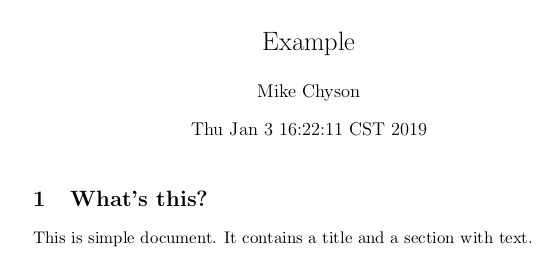
\includepdf[frame=true]{example}
\begin{figure}
  \centering
  \fbox{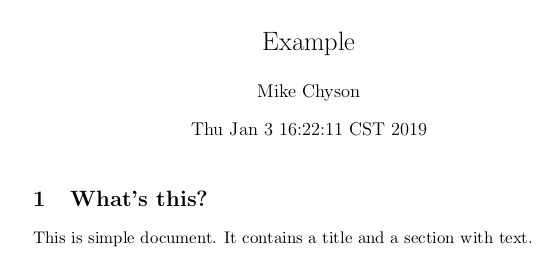
\includegraphics[width=0.8\textwidth]{example.png}}
  \caption{Example}
\end{figure}



Because the seperation of the format and the content, 
you do not specify the font size, font color, font family and so on.
Instead, you tell \LaTeX it is a \lcmd{title}, or \lcmd{author} or \lcmd{date} and so on.
\LaTeX format them for you.
As if there is a logical layer between the appearance and the content.


\section{Document Structure}
A \LaTeX document doesn't stand alone — commonly the document is based on a versatile template.
Such a fundamental template is called a class.
It provides customizable features, usually built for a certain purpose.

This first part of the document is called the preamble of the document. This is where we choose the class, specify properties, and in general, make document-wide definitions.

The first line starts with \verb|\documentclass|.
This word begins with a backslash; such a word is called a \keyword{command}.
We used commands to specify the class and to state document properties: \lcmd{title} , \lcmd{author} , and \lcmd{date}.


\begin{verbatim}
  preamble
  body
\end{verbatim}


\section{\LaTeX Command}
\lstset{language=TeX}
\begin{lstlisting}
  \command
  \command{argument}
  \command[optional argument]{argument}
\end{lstlisting}


\section{Comment}
The percent sing(\%) introduces a \keyword{comment}.




\section{Create Your Own Commands}

\subsection{With No Arguments}
\begin{lstlisting}
  \newcommand{\TUG}{TeX Users Group}
  \TUG
\end{lstlisting}

\subsection{With Arguments}

\begin{lstlisting}
  \newcommand{\keyword}[1]{\textbf{#1}}
  \keyword{declrations}
\end{lstlisting}

\subsection{With Optional Arguments}

\begin{lstlisting}
  \newcommand{\keyword2}[2][\bfseries]{{#1#2}}
  \keyword2[\itshape]{declarations}
\end{lstlisting}


\section{Breaking Lines}
\begin{lstlisting}
  \\                            % end a line
  \newline                      % has the same effect with \\
  \linebreak                    % tells LeTeX to end the line but to keep the full justification
  \\[3mm]                       % insert additional vertical space after the break depending on the value
  \linebreak[4]                 % can be used to influence the line break slightly or strongly:
%% If number is 0, a line break is allowed, 1 means it's desired, 2 and 3 mark more
%% insistent requests, and 4 will force it. The latter is the default behavior if no number
  %% was given.
  \nolinebreak
\end{lstlisting}


\section{Breaking Pages}
\begin{lstlisting}
  \pagebreak
  \newpage
  \nopagebreak
\end{lstlisting}


\section{Get Help}
Three ways to get help about the package:
\begin{itemize}
\item Use the \verb|texdoc| command:
  \begin{lstlisting}
    texdoc <package>
  \end{lstlisting}
\item Use the \verb|kpsewhich| command:
  \begin{lstlisting}
    kpsewhich <package>.sty
  \end{lstlisting}
\item Visit the website: \url{http://ctan.org/pkg}
\end{itemize}

  \chapter{Font}
\section{Shape}
\begin{table}[!h]
  \centering
  \caption{Font Command}
  \begin{tabular}{ccc}
    \toprule[1.5pt]
    \head{Command} & \head{Explaination} & \head{Output} \\
    \midrule
    \verb|\textbf| & bold font & \textbf{Example} \\
    \verb|\textit| & italic & \textit{Example} \\
    \verb|\textsl| & slated & \textsl{Example} \\
    \verb|\textsc| & small caps & \textsc{Example} \\
    \verb|\textup| & & \textup{Example} \\
    \verb|\textmd| & medium & \textmd{Example} \\
    \verb|\textnormal| & & \textnormal{Example} \\
    \bottomrule[1.5pt]
    
  \end{tabular}
  
\end{table}


\begin{table}[!h]
  \centering
  \caption{Font Declaration}
  \begin{tabular}{ccc}
    \toprule[1.5pt]
    \head{Declaration} & \head{Explaination} & \head{Output} \\
    \midrule
    \verb|\itshape| & italic & {\itshape Example} \\
    \verb|\bfseries| & bold font & {\bfseries Example} \\
    \verb|\slshape| & slated & {\slshape Example} \\
    \verb|\scshape| & small caps & {\scshape Example} \\
    \verb|\upshape| & & {\upshape Example} \\
    \verb|\mdseries| & medium & {\mdseries Example} \\
    \verb|\normalfont| & & {\normalfont Example} \\
    \bottomrule[1.5pt]
    
  \end{tabular}
  
\end{table}


\begin{table}[!hbp]
  \centering
  \caption{Font Emphasized}
  \begin{tabular}{ccc}
    \toprule[1.5pt]
    \head{Command} & \head{Explaination} & \head{Output} \\
    \midrule
    \verb|\emph| & emphasized & \emph{Example} \\
    \bottomrule[1.5pt]
  \end{tabular}
\end{table}
\clearpage
\section{Family}
\begin{table}[!hbp]
  \centering
  \caption{Font Family}
  \begin{tabular}{ccc}
    \toprule[1.5pt]
    \head{Command or Declariation} & \head{Explaination} & \head{Output} \\
    \midrule
    \verb|\textsf| & sans-serif & \textsf{Example} \\
    \verb|\texttt| & typewritter & \texttt{Example} \\
    \verb|\textrm| & Roman & \textrm{Example} \\
    \bottomrule[1.5pt]
  \end{tabular}
\end{table}

\clearpage

\section{Size}
\begin{table}[!hbp]
  \centering
  \caption{Font Size}
  \begin{tabular}{cc}
    \toprule[1.5pt]
    \head{Command} & \head{Output} \\
    \midrule
    \verb|\tiny| & \tiny{Example} \\
    \verb|\scriptsize| & \scriptsize{Example} \\
    \verb|\footnotesize| & \footnotesize{Example} \\
    \verb|\small| & \small{Example} \\
    \verb|\normalsize| & \normalsize{Example} \\
    \verb|\large| & \large{Example} \\
    \verb|\Large| & \Large{Example} \\
    \verb|\LARGE| & \LARGE{Example} \\
    \verb|\huge| & \huge{Example} \\
    \verb|\Huge| & \Huge{Example} \\
    \bottomrule[1.5pt]
  \end{tabular}
\end{table}


  

\chapter{Box}

\begin{lstlisting}
  \quad\parbox[b]{1.8cm}{this parbox is aligned at its bottom line}
\end{lstlisting}
\begin{tcolorbox}
\quad\parbox[b]{1.8cm}{this parbox is aligned at its bottom line}  
\end{tcolorbox}


\begin{lstlisting}
  \quad\parbox{1.5cm}{center-aligned parbox}
\end{lstlisting}
\begin{tcolorbox}
\quad\parbox{1.5cm}{center-aligned parbox}  
\end{tcolorbox}


\begin{lstlisting}
  \quad\parbox[t]{2cm}{another parbox aligned at its top line}
\end{lstlisting}
\begin{tcolorbox}
  \quad\parbox[t]{2cm}{another parbox aligned at its top line}
\end{tcolorbox}



\begin{lstlisting}
  \mbox{Hello World}
\end{lstlisting}

\begin{tcolorbox}
  \mbox{Hello World}
\end{tcolorbox}

  \chapter{Justification}
\begin{lstlisting}
\parbox{3cm}{\raggedright hello}    % \raggedright
{\centering hello}            % \centering
\begin{center}                % environment
  hello
\end{center}
\end{lstlisting}



  \chapter{Designing Pages}

\section{Defining the Overall Layout}
\begin{lstlisting}
  \usepackage[a4paper, inner=1.5cm, outer=3cm, top=2cm, bottom=3cm, bindingoffset=1cm, landscape]{geometry}
  %% paper=name
  %% paperwidth=7in
  %% paperheight=10in
  %% papersize={7in,10in}
  %% landscape
  %% portrait
  %% textwidth=140mm
  %% textheight=180mm
  %% lines=25
  %% includedhead % cause the header of the page to be included into the body area
  %% includefoot
  %% left=2cm
  %% right=2cm
  %% bindingoffset % reserves space on the left margin (one-size), respectively the inner margin (two-sided) for the binding

  %% default margin ratio:
  %% top:bottom = 2:3
  %% left:right = 1:1 for one-side documents
  %% inner:outer = 2:3 for two-side documents
\end{lstlisting}

\begin{lstlisting}
  \usepackage[onehalfspacing]{setspace}
  %% singlespacing, onehalfspacing, doublespacing
  %% \begin{spacing}{2.4}
  %% This text is stretched by a factor of 2.4.
  %% \end{spacing}
\end{lstlisting}


\begin{lstlisting}
  \documentclass[a4paper,12pt,twocolumn]{book} % the document class book, suitable for book-like documents
  %% book, report, article, slides, letter
  %% oneside or twoside
  %% openright or openany % only support book and report
  %% titlepage or notitlepage
  %% final or draft: If draft is set, then LaTeX will mark overfull lines with a black box, which is helpful in reviewing and improving the output.
  %% openbib : When this option is set, a bibliography would be formatted in open style instead of compressed style.
  %% fleqn : Causes displayed formulas to be left-aligned.
  %% leqno : For numbered displayed formulas, the number would be put to the left side. The right side is the default.
\end{lstlisting}


\section{Creating a Table of Contents}
\begin{lstlisting}
  \tableofcontents
\end{lstlisting}

\section{Designing Headers and Footers}
\begin{lstlisting}
  \usepackage{fancyhdr}
  \fancyhf{}
  \fancyhead[LE]{\leftmark}
  \fancyhead[RO]{\nouppercase{\rightmark}}
  \fancyfoot[LE,RO]{\thepage}
  \pagestyle{fancy}
\end{lstlisting}

  \chapter{Footnotes}

\begin{lstlisting}
  \footnote{hello world}
  \section[title without footnote]{This is a section\protect\footnote{section footnote}}

  \footnote[number]{text}

  \footnotemark[number] % produces a superscripted number in the text as a
  % footnote mark. If the optional argument wasn't given, it's also stepping and using
  % the internal footnote counter. No footnote will be generated.

  \footnotetext[number]{text} % generates a footnote without putting a
  % footnote mark into the text without stepping the internal footnote counter.

  \footnoterule % used to alter the footnote line

  \renewcommand{\footnoterule}{\noindent\smash{\rule[3pt]{\textwidth}{0.4pt}}}
  % \rule[raising]{width}{height} draws a line, here 0.4 pt thick, and as wide as the text, raised a bit by 3 pt.
  % \smash , let the line pretend to have a height and a depth of zero, so it's occupying no vertical space at all.
\end{lstlisting}

Example:
\begin{lstlisting}
  Hello World\footnote{hello world}
\end{lstlisting}
\begin{tcolorbox}
Hello World\footnote{hello world}.  
\end{tcolorbox}




  \chapter{Lists}
\section{Bulleted Lists}

\begin{lstlisting}
  \begin{itemize}
  \item geometry
  \item amsmath
  \end{itemize}
\end{lstlisting}

\begin{tcolorbox}
  \begin{itemize}
  \item geometry
  \item amsmath
  \end{itemize}
\end{tcolorbox}

\section{Numbered Lists}
\begin{lstlisting}
  \begin{enumerate}
  \item geometry
  \item amsmath
  \end{enumerate}
\end{lstlisting}

\begin{tcolorbox}
  \begin{enumerate}
  \item geometry
  \item amsmath
  \end{enumerate}
\end{tcolorbox}



\section{Definition Lists}
\begin{lstlisting}
  \begin{description}
  \item[paralist] provides compact lists and list versions that
    can be used within paragraphs, helps to customize labels and
    layout
  \item[enumitem] gives control over labels and lengths
    in all kind of lists
  \item[mdwlist] is useful to customize description lists, it
    even allows multi-line labels. It features compact lists and
    the capability to suspend and resume.
  \item[desclist] offers more flexibility in definition list
  \item[multenum] produces vertical enumeration in multiple
    columns
  \end{description}
\end{lstlisting}

\begin{tcolorbox}
  \begin{description}
  \item[paralist] provides compact lists and list versions that
    can be used within paragraphs, helps to customize labels and
    layout
  \item[enumitem] gives control over labels and lengths
    in all kind of lists
  \item[mdwlist] is useful to customize description lists, it
    even allows multi-line labels. It features compact lists and
    the capability to suspend and resume.
  \item[desclist] offers more flexibility in definition list
  \item[multenum] produces vertical enumeration in multiple
    columns
  \end{description}
\end{tcolorbox}

  \chapter{Tables}

\begin{lstlisting}
  \newcommand{\head}[1]{\textnormal{\textbf{#1}}}
  \begin{tabular}{ccc}
    \hline
    \head{Command} & \head{Declaration} & \head{Output} \\
    \hline
    \verb|\textrm| & \verb|\rmfamily| & \rmfamily Example text \\
    \verb|\textsf| & \verb|\sffamily| & \sffamily Example text \\
    \verb|\texttt| & \verb|\ttfamily| & \ttfamily Example text \\
    \hline
  \end{tabular}
\end{lstlisting}

\begin{tcolorbox}
  \begin{tabular}{ccc}
    \hline
    \head{Command} & \head{Declaration} & \head{Output} \\
    \hline
    \verb|\textrm| & \verb|\rmfamily| & \rmfamily Example text \\
    \verb|\textsf| & \verb|\sffamily| & \sffamily Example text \\
    \verb|\texttt| & \verb|\ttfamily| & \ttfamily Example text \\
    \hline
  \end{tabular}
\end{tcolorbox}


\newpage
\begin{lstlisting}

  \usepackage{booktabs} % toprule, midrule, bottomrule

  \begin{tabular}{ccc}
    \toprule[1.5pt] % British typesetters call a line a rule
    \head{Command} & \head{Declaration}& \head{Output}\\
    \midrule %
    \verb|\textrm| & \verb|\rmfamily| & \rmfamily Example text \\
    \verb|\textsf| & \verb|\sffamily| & \sffamily Example text \\
    \verb|\texttt| & \verb|\ttfamily| & \ttfamily Example text \\
    \bottomrule[1.5pt] %
  \end{tabular}

\end{lstlisting}

\begin{tcolorbox}
  
  \begin{tabular}{ccc}
    \toprule[1.5pt] % British typesetters call a line a rule
    \head{Command} & \head{Declaration}& \head{Output}\\
    \midrule %
    \verb|\textrm| & \verb|\rmfamily| & \rmfamily Example text \\
    \verb|\textsf| & \verb|\sffamily| & \sffamily Example text \\
    \verb|\texttt| & \verb|\ttfamily| & \ttfamily Example text \\
    \bottomrule[1.5pt] %
  \end{tabular}

\end{tcolorbox}


\begin{tcolorbox}
  To avoid the table exceed out the page:
\begin{verbatim}
    \resizebox{\textwidth}{!}{
      ...
    }
  
\end{verbatim}


\end{tcolorbox}


To wrap automatically in cell, use the \verb|p{width}| parameter.
For example:
\begin{lstlisting}
  
\begin{table}[htb!]
  \centering
  \begin{tabular}{p{0.3\columnwidth}p{0.3\columnwidth}p{0.3\columnwidth}}
    \toprule{}
    & \head{advantage} & \head{disadvantage} \\
    \midrule
    multiple processes & each process runs independently & communication and data sharing can be inconvenient \\
    multiple threads & can communicate simply by data sharing & more complex than single-threaded program\\
    \bottomrule
  \end{tabular}
  \caption{multiple processes and multiple threads}
\end{table}
\end{lstlisting}


\begin{table}[htb!]
  \centering
  \begin{tabular}{p{0.3\columnwidth}p{0.3\columnwidth}p{0.3\columnwidth}}
    \toprule{}
    & \head{advantage} & \head{disadvantage} \\
    \midrule
    multiple processes & each process runs independently & communication and data sharing can be inconvenient \\
    multiple threads & can communicate simply by data sharing & more complex than single-threaded program\\
    \bottomrule
  \end{tabular}
  \caption{multiple processes and multiple threads}
\end{table}






  \chapter{Figure}

\begin{lstlisting}
  \usepackage{graphicx}
  \begin{figure}
    \centering
    
\includegraphics[width=0.8\textwidth]{zm.jpg}   % include picture
  \end{figure}
\end{lstlisting}


\begin{figure}
  \centering
  
\includegraphics[width=0.8\textwidth]{zm.jpg}   % include picture
\end{figure}





  \chapter{Cross Referencing}
\begin{lstlisting}
  \label % mark the label
  \ref % refer after marking
  \pageref
  % notice, typeset twice to produce the corrent reference

  % If the \label command appeared in ordinary text, then the current sectional unit,
  % like the chapter or the section, would be assigned.
  % If the \label would be placed within a numbered environment, that environment
  % would be assigned to the key.

  \newcommand{\fullref}[1]{\ref{#1} on page~\pageref{#1}}
\end{lstlisting}

For example:

\begin{lstlisting}
  Hello World\label{hello-label}

  Refer to \ref{hello-label}
\end{lstlisting}

\begin{tcolorbox}
Hello World\label{hello-label}

Refer to \ref{hello-label}
\end{tcolorbox}


  \chapter{Content}

\begin{table}[!ht]
  \caption{Content}
  \centering
  \begin{tabular}{cc}
    \toprule[1.5pt]
    \head{Command} & \head{Level} \\
    \midrule
    \verb|\part| & -1 (book and report class) \\
    \verb|\chapter| & 0 (not available in article) \\
    \verb|\section| & 1 \\
    \verb|\subsection| & 2 \\
    \verb|\subsubsection| & 3 \\
    \verb|\paragraph| & 4 \\
    \verb|\subparagraph| & 5 \\
    \bottomrule[1.5pt]
  \end{tabular}
\end{table}



  \chapter{Math}

\section{Basic Formula}

\begin{lstlisting}
  \section*{Quadratic equations}
  \begin{equation}
    \label{quad}
    ax^2 + bx + c = 0,
  \end{equation}
  where \( a, b\) and \( c \) are constants and \( a \neq 0 \),
  has two solutions for the variable \( x \):
  \begin{equation}
    \label{root}
    x_{1,2} = \frac{-b \pm \sqrt{b^2 -4ac}}{2a}.
  \end{equation}
  If the \emph{discriminant} \( \Detla \) with
  \[ \Delta = b^2 - 4ac \]
  is zero, then the equation (\ref{quad}) has a double solution:
  (\ref{root}) becomes
  \[ x = - \frac{b}{2a}. \]
\end{lstlisting}

% \begin{tcolorbox}
%   \section*{Quadratic equations}
%   \begin{equation}
%     \label{quad}
%     ax^2 + bx + c = 0,
%   \end{equation}
%   where \( a, b\) and \( c \) are constants and \( a \neq 0 \),
%   has two solutions for the variable \( x \):
%   \begin{equation}
%     \label{root}
%     x_{1,2} = \frac{-b \pm \sqrt{b^2 -4ac}}{2a}.
%   \end{equation}
%   If the \emph{discriminant} \( \Detla \) with
%   \[ \Delta = b^2 - 4ac \]
%   is zero, then the equation (\ref{quad}) has a double solution:
%   (\ref{root}) becomes
%   \[ x = - \frac{b}{2a}. \]

% \end{tcolorbox}


\section{Expressions within Text}
LaTeX provides the math environment in-text formulas:

\begin{lstlisting}
  \begin{math}
    expression
  \end{math}
\end{lstlisting}

LaTeX offers an alias that's doing the same:

\begin{lstlisting}
  \( expression \)
\end{lstlisting}

A third way is by using a shortcut, coming from TeX:

\begin{lstlisting}
  $expression$
\end{lstlisting}

For example:
\begin{tcolorbox}
  \begin{lstlisting}
    This is an equation: $x^2 + x = 10$
  \end{lstlisting}
  This is an equation: $x^2 + x = 10$
\end{tcolorbox}

\section{Displaying Formula}

\begin{lstlisting}
  \begin{displaymath}
    expression                  % displayed formula, centered
  \end{displaymath}
\end{lstlisting}


There are shortcuts:
\begin{lstlisting}
  \[
    expression
  \]
\end{lstlisting}

\begin{lstlisting}
  $$
  expression
  $$
\end{lstlisting}



For example:
\begin{tcolorbox}
  \begin{lstlisting}
    \begin{displaymath}
      x^2 + x = 10
    \end{displaymath}
  \end{lstlisting}
  \begin{displaymath}
    x^2 + x = 10
  \end{displaymath}

\end{tcolorbox}


\section{Numbering Equations}
\begin{tcolorbox}
  \begin{lstlisting}
    \begin{equation}
      \label{newton}
      F = ma^2
    \end{equation}
    Newton's law: \eqref{newton}.
  \end{lstlisting}
  \begin{equation}
    \label{newton}
    F = ma^2
  \end{equation}
  Newton's law: \eqref{newton}.

\end{tcolorbox}



  \chapter {Larger Document}

If you are writing a book, it is better to split the book into several parts.

For example:

\begin{verbatim}
  \documentclass{book}
  \input{preamble}

  \hypersetup{pdfauthor={Li Mingming},
    pdftitle={The Big Book of \LaTeX},
    pdfsubject={Introduction to \LaTeX and how to use it},
    pdfkeywords={latex}}

  \begin{document}

  \frontmatter
  \include{title}
  \include{dedication}
  \tableofcontents
  \listoftables
  \listoffigures
  \mainmatter
  \include{environment}
  \include{what-is-latex}
  \include{latex-base}
  \include{font}
  \include{box}
  \include{justification}
  \include{designing-pages}
  \include{footnote}
  \include{list}
  \include{table}
  \include{figure}
  \include{cross-referencing}
  \include{content}
  \include{math}
  \include{large-document}
  \backmatter
  \bibliographystyle{plainnat}
  \bibliography{tex}


  \end{document}
  
\end{verbatim}






  \backmatter
  \bibliographystyle{plainnat}
  \bibliography{tex}


  \end{document}
  
\end{verbatim}






  \backmatter
  \bibliographystyle{plainnat}
  \bibliography{tex}


  \end{document}
  
\end{verbatim}






  \backmatter
  \bibliographystyle{plainnat}
  \bibliography{tex}


  \end{document}
  
\end{verbatim}





